% !TeX program = pdflatex
\documentclass[border=6pt]{standalone}
\usepackage{tikz}
\usetikzlibrary{arrows.meta, positioning, calc}

\definecolor{MediumRed}{rgb}{0.925, 0.345, 0.345}
\definecolor{MediumGreen}{rgb}{0.37, 0.7, 0.66}
\definecolor{MediumBlue}{rgb}{0.015, 0.315, 0.45}
\definecolor{DarkBlue}{rgb}{0.05, 0.15, 0.35}

\begin{document}
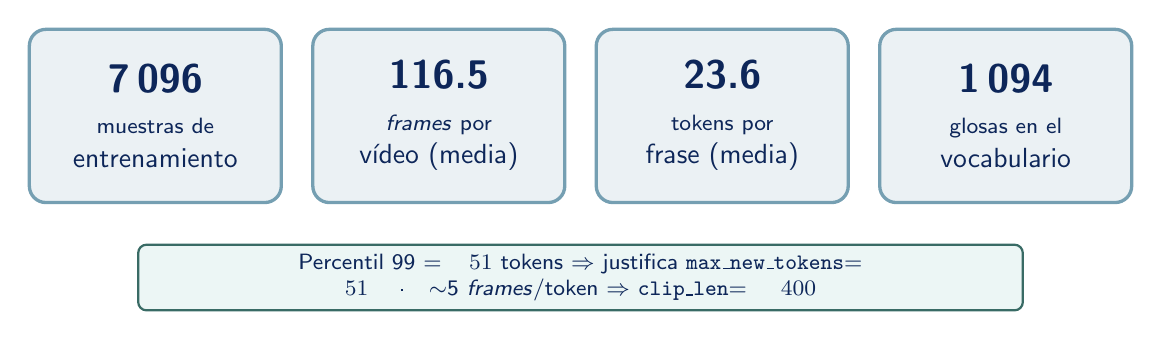
\begin{tikzpicture}[font=\sffamily,
    stat/.style={draw=MediumBlue!55, very thick, rounded corners=6pt, fill=MediumBlue!8,
        text=DarkBlue, align=center, minimum width=3.2cm, minimum height=2.2cm}]

\node[stat] (a) at (0,0)
    {{\Large\bfseries 7\,096}\\[3pt]\footnotesize muestras de\\ entrenamiento};
\node[stat] (b) at (3.6,0)
    {{\Large\bfseries 116.5}\\[3pt]\footnotesize \emph{frames} por\\ vídeo (media)};
\node[stat] (c) at (7.2,0)
    {{\Large\bfseries 23.6}\\[3pt]\footnotesize tokens por\\ frase (media)};
\node[stat] (d) at (10.8,0)
    {{\Large\bfseries 1\,094}\\[3pt]\footnotesize glosas en el\\ vocabulario};

\node[draw=MediumGreen!60!black, thick, rounded corners=3pt, fill=MediumGreen!12, text=DarkBlue,
      font=\sffamily\footnotesize, align=center, text width=11.0cm, below=0.5cm of b, xshift=1.8cm]
    {Percentil 99 $=51$ tokens $\Rightarrow$ justifica \texttt{max\_new\_tokens}$=51$
     \quad·\quad $\sim$5 \emph{frames}/token $\Rightarrow$ \texttt{clip\_len}$=400$};

\end{tikzpicture}
\end{document}
